\documentclass[submit,techrep,noauthor]{ipsj}

\usepackage{amsmath,amssymb,amsfonts}
\usepackage{cite}
\usepackage[japanese]{babel}
\usepackage[scaled]{beramono}
\usepackage{booktabs}
\usepackage[T1]{fontenc}
\usepackage[dvipdfmx]{graphicx}
\usepackage[utf8]{inputenc}
\usepackage{listings}
\usepackage[all, warning]{onlyamsmath}
\usepackage[subrefformat=parens]{subcaption}
\usepackage{url}

\def\Underline{\setbox0\hbox\bgroup\let\\\endUnderline}
\def\endUnderline{\vphantom{y}\egroup\smash{\underline{\box0}}\\}
\def\|{\verb|}

\begin{document}


\title{ベクトル型スーパーコンピュータ「AOBA-S」の性能評価}

\etitle{Performance Evaluation of a Vector Supercomputer ``AOBA-S''}

\affiliate{CSC}{東北大学サイバーサイエンスセンター}
\affiliate{NEC}{日本電気株式会社}
\affiliate{TU}{東北大学大学院情報科学研究科}
\affiliate{TDU}{東京電機大学}

\author{高橋 慧智}{Keichi Takahashi}{CSC,TU}[keichi@tohoku.ac.jp]
\author{藤本 壮也}{Soya Fujimoto}{NEC}[s-fujimoto@nec.com]
\author{長瀬 悟}{Satoru Nagarase}{NEC}[s.nagase@nec.com]
\author{磯部 洋子}{Yoko Isobe}{NEC}[y-isobe-pi@nec.com]
\author{下村 陽一}{Yoichi Shimomura}{CSC,TU}[shimomura32@tohoku.ac.jp]
\author{江川 隆輔}{Ryusuke Egawa}{TDU}[egawa@mail.dendai.ac.jp]
\author{滝沢 寛之}{Hiroyuki Takizawa}{CSC,TU}[takizawa@tohoku.ac.jp]

\begin{abstract}
東北大学サイバーサイエンスセンターは,2023年8月よりベクトル型スーパーコンピュータ「AOBA-S」の運用を
開始した.AOBA-Sは第3世代ベクトルエンジン (VE30) をノードあたり8基搭載した計504ノードから構成され,
理論演算性能は21.05\,PFLOP/s,メモリ帯域幅は9.97\,PB/sに達する世界最大規模のベクトル型
スーパーコンピュータである.本稿ではAOBA-Sの設計を概説し,運用開始に先駆けて実施したAOBA-Sの
初期性能評価の結果について報告する.
\end{abstract}

\begin{eabstract}
Cyberscience Center, Tohoku Unviversity has started the operation of a new vector supercomputer 
``AOBA-S'' in August 2023. AOBA-S comprises of 504 compute nodes each equipped with eight
third-generation Vector Engine (VE30) cards. Its peak compute performance reachaes 21.05\,PFLOP/s
and its peak memory bandwidth is 9.97\,TB/s -- making it the world's largest vector super computer as
of writing this paper. In this paper, we describe the basic design of AOBA-S and report the
results of the initial performance evaluation that we have conducted prior to the operation start of
AOBA-S.
\end{eabstract}

%
%\begin{jkeyword}
%情報処理学会論文誌ジャーナル,\LaTeX,スタイルファイル,べからず集
%\end{jkeyword}
%
%\begin{ekeyword}
%IPSJ Journal, \LaTeX, style files, ``Dos and Dont's'' list
%\end{ekeyword}

\maketitle

\section{はじめに}

図\ref{fig:node}にAOBA-Sを構成するSX-Aurora C401-8ノードのアーキテクチャを示す.
各ノードの中核にはAMD EPYC 7763プロセッサがあり,合計256GBのメモリを搭載している.
各ノードには8基のVector Engine Type 30Aプロセッサが搭載されている.
2基ずつ1つのPCIeスイッチに接続されており,各PCIeスイッチがルートコンプレックスに接続している.

図\ref{fig:ve30}にVE30プロセッサの概要図を示す.

前世代のVE Type 20Aと比較すると,ベクトルコアあたりの計算性能とメモリアクセス性能を同一である一方,
コア数が10コアから16コアへ1.6倍に増加している.また,コア数の増加に応じてメモリ帯域幅も1.53\,TB/sから
2.54\,TB/sへ1.6倍に向上している.さらに,メモリ容量は48\,GBから96\,GBへ2倍に拡大され,LLCの容量は
16\,MBから64\,MBへ4倍に拡大している.

相互結合網にはInfiniBand
NDRを採用しており,フルバイセクションバンド幅およびノンブロッキングの2段Fat-treeトポロジによって
計算ノードおよびストレージノードが接続されている.計算ノード側のHCAにはInfiniBand NDR
200GのHCAが2枚搭載されている.計算ノード群2ラックにつき1つのInfiniBandスイッチに接続している.
計算ノードのバイセクションバンド幅は,204.8\,Tbpsに達する.

ストレージにはDDN社製ES400NVX2アプライアンスを採用している.
1基のES400NVX2がLustre MDS/MDTとして動作し,もう1基のES400NVX2がOSS/OSTとして動作する.
OSS/OST用ES400NVX2には4基のSS9012エンクロージャが接続され,合計332本の7200rpm ニアラインSAS
HDDを搭載している.各ES400NVX2は8本のInfiniBand HDRリンクによって相互結合網に接続している.

\begin{figure}
  \centering
  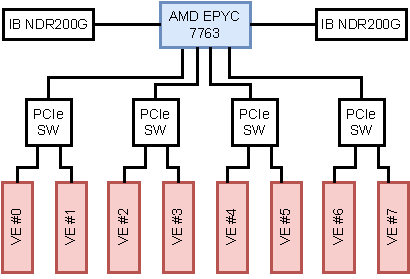
\includegraphics{figs/node_arch.pdf}
  \caption{SX-Aurora TSUBASA C401-8の構成}\label{fig:node}
\end{figure}

\begin{figure}
  \centering
  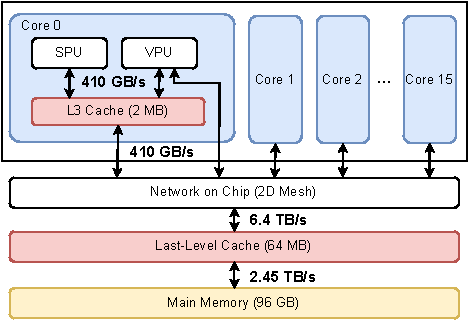
\includegraphics{figs/ve30_memory_hierarchy.pdf}
  \caption{VE30の概要図~\cite{Takahashi2023}}\label{fig:ve30}
\end{figure}


\section{MPI通信性能}

OSU Micro-Benchmarks
7.2\footnote{\url{https://mvapich.cse.ohio-state.edu/benchmarks/}}を用いてMPI通信の性能を計測した.
NCC 5.0.1でコンパイルし,MPIライブラリにNEC MPI 3.4.0を用いた.
測定にあたっては,(1) 同一PCIeスイッチに接続されたVE間,(2)
同一ノード内の異なるPCIeスイッチに接続されたVE間,(3) 同一ラックの異なるノードに接続されたVE間,
の3パターンを計測した.

\subsection{1対1通信}

図\ref{fig:mpi-lat}に\verb|osu_latency|ベンチマークで計測したMPI 1対1通信のレイテンシを示す.
1.55$\mu$s

\begin{figure}
  \centering
  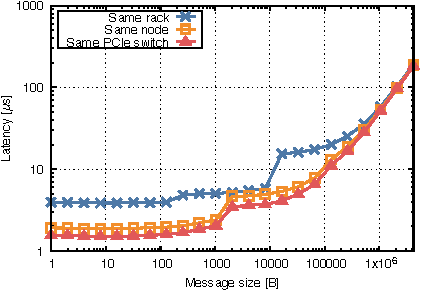
\includegraphics{figs/mpi_latency.pdf}
  \caption{MPI 1対1通信のレイテンシ}\label{fig:mpi-lat}
\end{figure}

\begin{figure}
  \centering
  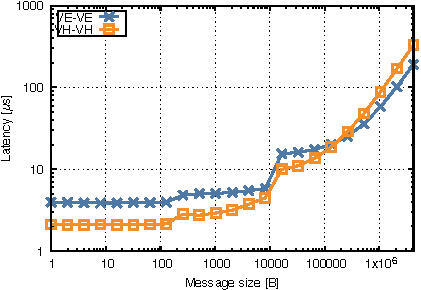
\includegraphics{figs/mpi_latency_vhve.pdf}
  \caption{MPI 1対1通信のレイテンシ}\label{fig:mpi-lat-vh}
\end{figure}

図\ref{fig:mpi-lat}に\verb|osu_bandwidth|ベンチマークで計測したMPI 1対1通信のスループットを示す.

PCIe Gen 4 $\times$16の実効帯域幅31.508\,GB/sである.73.4\%

\begin{figure}
  \centering
  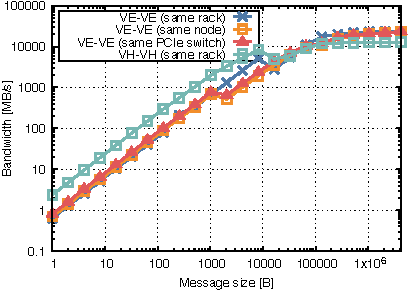
\includegraphics{figs/mpi_bandwidth.pdf}
  \caption{MPI 1対1通信のスループット}\label{fig:bw}
\end{figure}

\begin{figure}
  \centering
  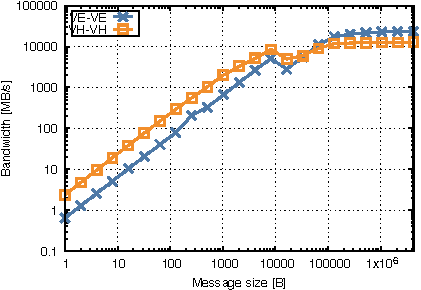
\includegraphics{figs/mpi_bandwidth_vhve.pdf}
  \caption{MPI 1対1通信のスループット}\label{fig:bw-vh}
\end{figure}

\section{ストレージ性能}

IOR 3.3.0を用いて並列ファイルシステムの性能を計測した.1VEにつきIORを1プロセスを起動し,
計測に用いたコマンドは,
\texttt{ior -w -r -a POSIX -F -Q 8 -C -e -g -b 16m -t 4m -s 250 -i 3}である.
書き込み時のページキャッシュの効果を排除するため,\texttt{-e}オプションによってwrite完了時に
\texttt{fsync()}を呼び出している.また,読み込み時のページキャッシュの効果を排除するため,書き込みを
実行するVEと読み込みを実行するVEをずらす\texttt{-C}オプションを指定している.また,
同一VHに接続されたVEはVH側においてページキャッシュを共有しているため,異なるVHを
\texttt{-Q 8}

\begin{figure}
  \centering
  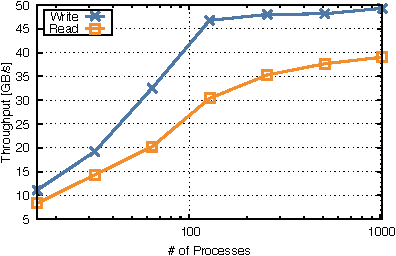
\includegraphics{figs/ior.pdf}
  \caption{並列ファイルシステムのスループット}\label{fig:ior}
\end{figure}

\subsection*{謝辞}

性能評価にご協力いただいた東北大学情報部デジタルサービス支援課および日本電気株式会社の皆様に
感謝いたします.

\bibliographystyle{IEEEtran}
\bibliography{references}

\end{document}
